\section{Daten}


\subsection{Datenquellen}
Es gibt keine frei zugänglichen umfassenden Datensätze für Sprachidentifikation. Datensätze, wie das \textit{NIST Language Recognition Evaluation}\cite{nist}, sind nur unter teuren Gebühren zugänglich. Wie verwandte Arbeiten empfehlen \cite{iLID}, wird darum ein eigener Datensatz zusammengestellt. Es werden gleichmässig Daten zu den Sprachen Deutsch, Englisch, und Französisch gesammelt. Die Daten stammen vom \textit{Voxforge}\cite{voxforge} Datensatz, von \textit{Youtube}\cite{youtube} und von \textit{Librivox}\cite{librivox}.

\paragraph{Voxforge} ist ein open-source Datensatz für Spracherkennung. Es besteht aus vielen kurzen (1-10s), von Benutzern hochgeladenen, Audiodateien. Die englische Sprache dominiert mit rund 120h Audio den Datensatz. Über alle drei Sprachen verteilt sind 190 Stunden Ton verfügbar. Die Audioqualität variiert je nach Benutzer.

Die Sprache ist langsam und deutlich verständlich. Sie hört sich eher künstlich an im Vergleich zu einem natürlichen Gespräch. Die Anzahl unterschiedlicher Sprecher ist gering.

\paragraph{Youtube}dient als Quelle für abwechslungsreiche Sprache. Es werden populären Nachrichtenkanäle wie CNN, ZDF, etc. verwendet (Siehe Tabelle \ref{tab:channels}). Die Aufnahmen werden oft von diversen Hintergrundgeräuschen begleitet und die Variation der Sprecher gross, da oft fremde Gäste eingeladen werden. Kehrseite ist, dass nicht garantiert werden kann, dass alle Aufnahmen tatsächlich die richtige Sprache beinhalten. Sendepausen und fremdsprachige Interviews kommen vereinzelt vor.
\begin{table}[h]
        \centering
        \begin{tabular}[t]{l || l}
        Sprache & Kanäle \\
        \hline \hline
        Französisch & France24, FranceInfo, BFMTV\\
        Deutsch & NDR, ZDF, DW\\
        Englisch & CNN,  BBC
        \end{tabular}
        \caption{Youtube Kanäle}
        \label{tab:channels}
\end{table}

\paragraph{Librivox} ist ein öffentlich abrufbarer Hörbuch Datensatz. Anstatt selbst Hörbücher zu selektieren, wird eine vorgefertigte Selektion verwendet \cite{librivox-compilation}. Verfügbar sind sieben Stunden Aufnahmen mit 90 verschiedenen Sprechern.


\subsection{Daten Auswahl}
Die Modelle werden grundsätzlich mit den Daten von Voxforge und Youtube trainiert und ausgewertet. Die Verwendung von zwei unterschiedlichen Datenquellen minimiert die \textit{Stichprobenverzerrung}. Stichprobenverzerrung bedeutet, dass der Datensatz nicht repräsentativ für alle Sprachaufnahmen ist. Bei Voxforge ist zum Beispiel die Gefahr, dass das Modell sich an die geringe Anzahl Sprecher überanpasst. Anstatt die Sprache zu erkennen, könnte das Modell das Mikrofon des Sprechers identifizieren und jedem Sprecher eine Sprache zuordnen. Die Leistung des Modells für neue Sprecher wäre dann nicht besser als ein Zufallsgenerator.
\\
Um die Stichprobenverzerrung zu messen, werden die Modelle zusätzlich auf dem Librivox Datensatz ausgewertet. Die Daten von Librivox teilen keine systematischen \say{Fehler} wie zum Beispiel Sprecher mit den Trainingsdaten. Das Librivox-Testset besteht aus insgesamt 8.5 Stunden Aufnahmen.
\\
Von Youtube und Voxforge werden gemeinsam 139 Stunden Audiodaten heruntergeladen, was 100'000 5s Aufnahmen entspricht. Die Datenmenge wird bewusst klein gehalten, weil grössere Datenmengen ressourcenaufwändiger und ineffizienter wären. Die einzelnen Sprachen und Quellen sind zu gleichen Teilen repräsentiert. 
\\
Die Daten werden weiter in 80\% Trainingsdaten, 10\% Testdaten und 10\% \textit{Validationset} gespalten. Das Validationset wird verwendet um während dem Training zu beobachten, wie das Modell auf neue Daten reagiert. Die \textit{Hyperparamter} \index{Hyperparameter}(Parameter die das Netzwerk nicht selber lernen kann, z.B. die Anzahl Knoten) werden manuell so angepasst, dass das Netzwerk möglichst gut auf dem Validationset abschneidet. Tabelle \ref{tab:data} gibt eine Übersicht über die Verteilung der Daten.
\begin{table}[]
	\centering
	\begin{tabular}{llll}
	\hline
	Netz          & Voxforge & Youtube & Librivox \\ \hline
	Trainingset   & 56h      & 56h     & -        \\
	Validationset & 7h       & 7h      & -        \\
	Testset       & 7h       & 7h      & 8.5h       \\ \hline
	\end{tabular}
	\caption{Daten Verteilung}
	\label{tab:data}
\end{table}


\subsection{Preprocessing}
Sprache besteht aus Wörtern und verschiedene Sprachen unterscheiden sich grundsätzlich durch einen anderen Wortschatz. Wörter lassen sich wiederum in verschiedene Laute spalten. Sprachen unterscheiden sich also auch an den verschiedenen Abfolgen von Lauten, manchmal sogar an den verwendeten Lauten selbst. Die kleinste relevante Einheit für Spracherkennung, sowohl für den Menschen wie die Maschine, ist wahrscheinlich ein Laut.

Wenn der Computer mit dem Mikrofon aufnimmt, misst er kleinste Druckunterschiede, bzw. Schallwellen. Eine unkomprimierte Audiodatei zeigt den Schalldruck über die Länge der Aufnahme, siehe Abbildung \ref{img:preprocessing} \textit{(oben)}.
Die einzelne Schallwelle ist für den Menschen nicht erkennbar, deshalb ist sie auch für die Sprache von keiner Bedeutung. Erst mehrere Schallwellen, bzw. die daraus folgende Frequenz lässt sich als Laut hören. 
Das Verfahren um aus einer Schallwelle die unterschiedlichen Frequenzen zu bestimmen heisst \textit{Fourier-Transformation} \cite{fourrier}. Falls dem Netzwerk als Eingabe rohe Schallwellen gefüttert werden, muss es dieses Verfahren erlernen, um dann aus den Lauten die Sprache erkennen zu können. Allerdings ist die Fourrier-Transformation zu erlernen ein zusätzlicher Aufwand und fordert den Computer darum mehr. Um dem Algorithmus die Aufgabe zu erleichtern, kann man ihm darum als Eingabe die berechneten Laute anstatt der rohen Schallwelle geben.

Die Prozedur dem Algorithmus bereits vorgerechnete Werte zu füttern, heisst \textit{Preprocessing} \index{Preprocessing}und ist weit verbreitet im Feld von \textit{Machine learning}. Das Vorrechnen ist unter dem Namen \index{Feature Engineering}\textit{Feature Engineering} bekannt. \textit{Features}, also Merkmale z.B. Laute werden aus den Rohen Daten extrahiert. \parencite[vgl.][]{chollet}

\subsubsection{Spektrogramme} \index{Spektrogramme}
\begin{figure}[hbt]
	\centering
		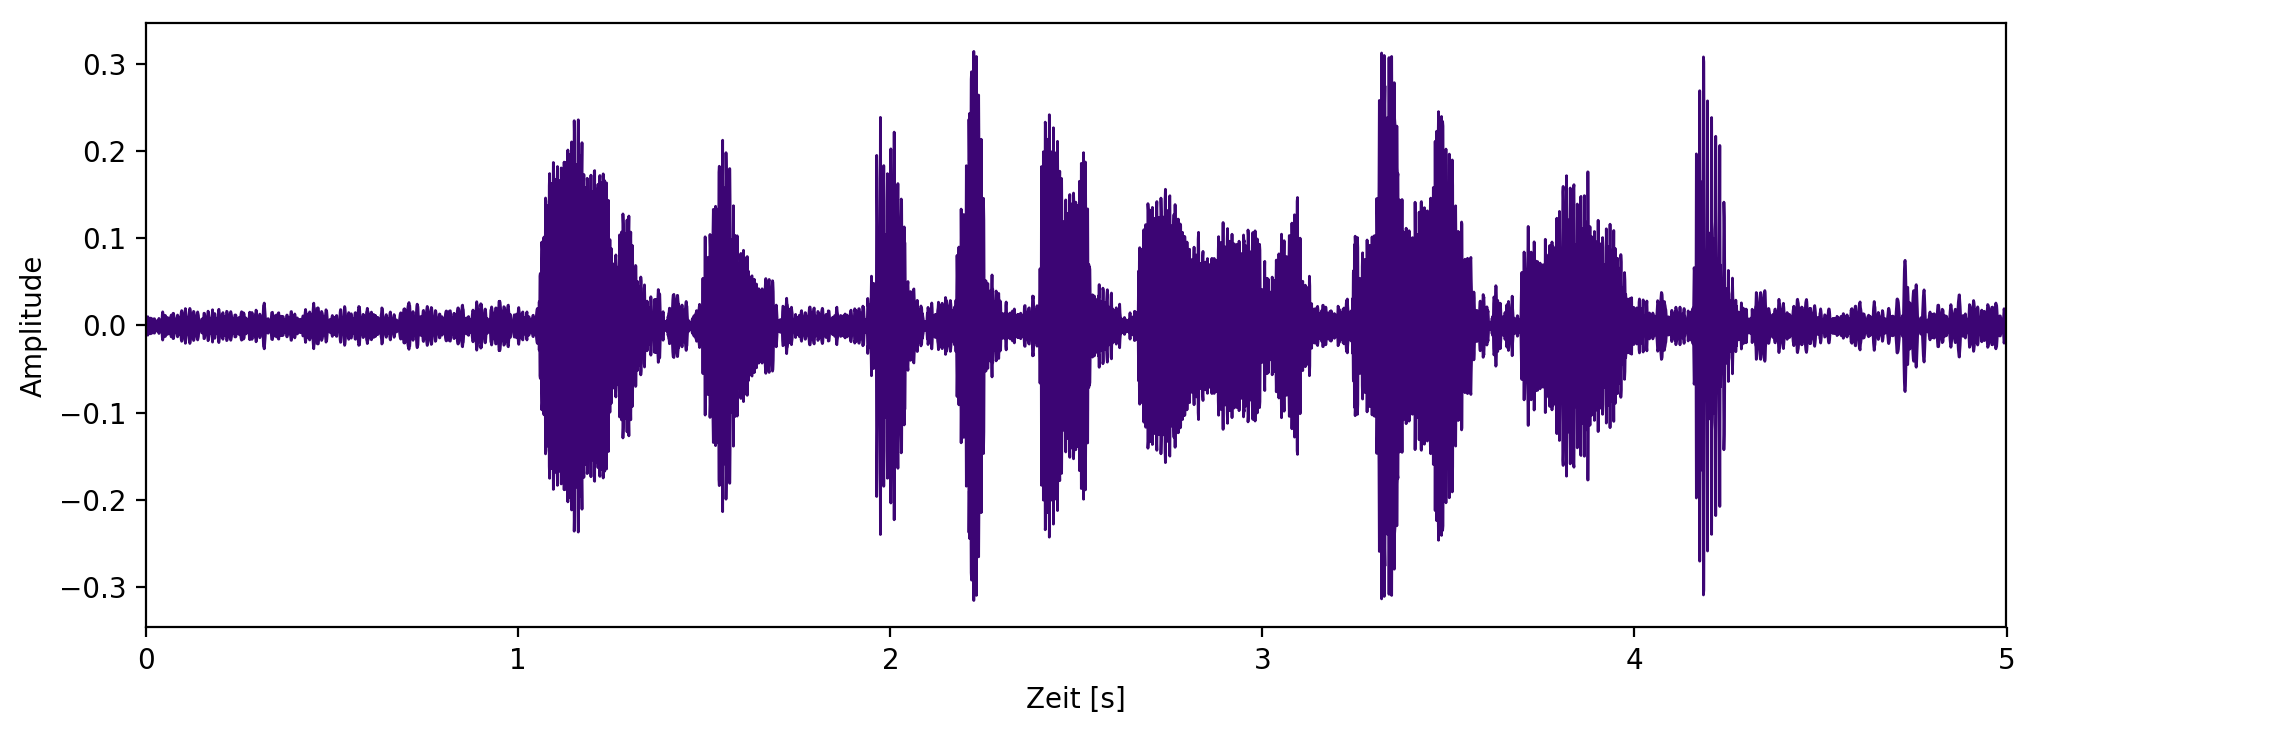
\includegraphics[width=0.8\textwidth]{assets/audio_raw.png}
		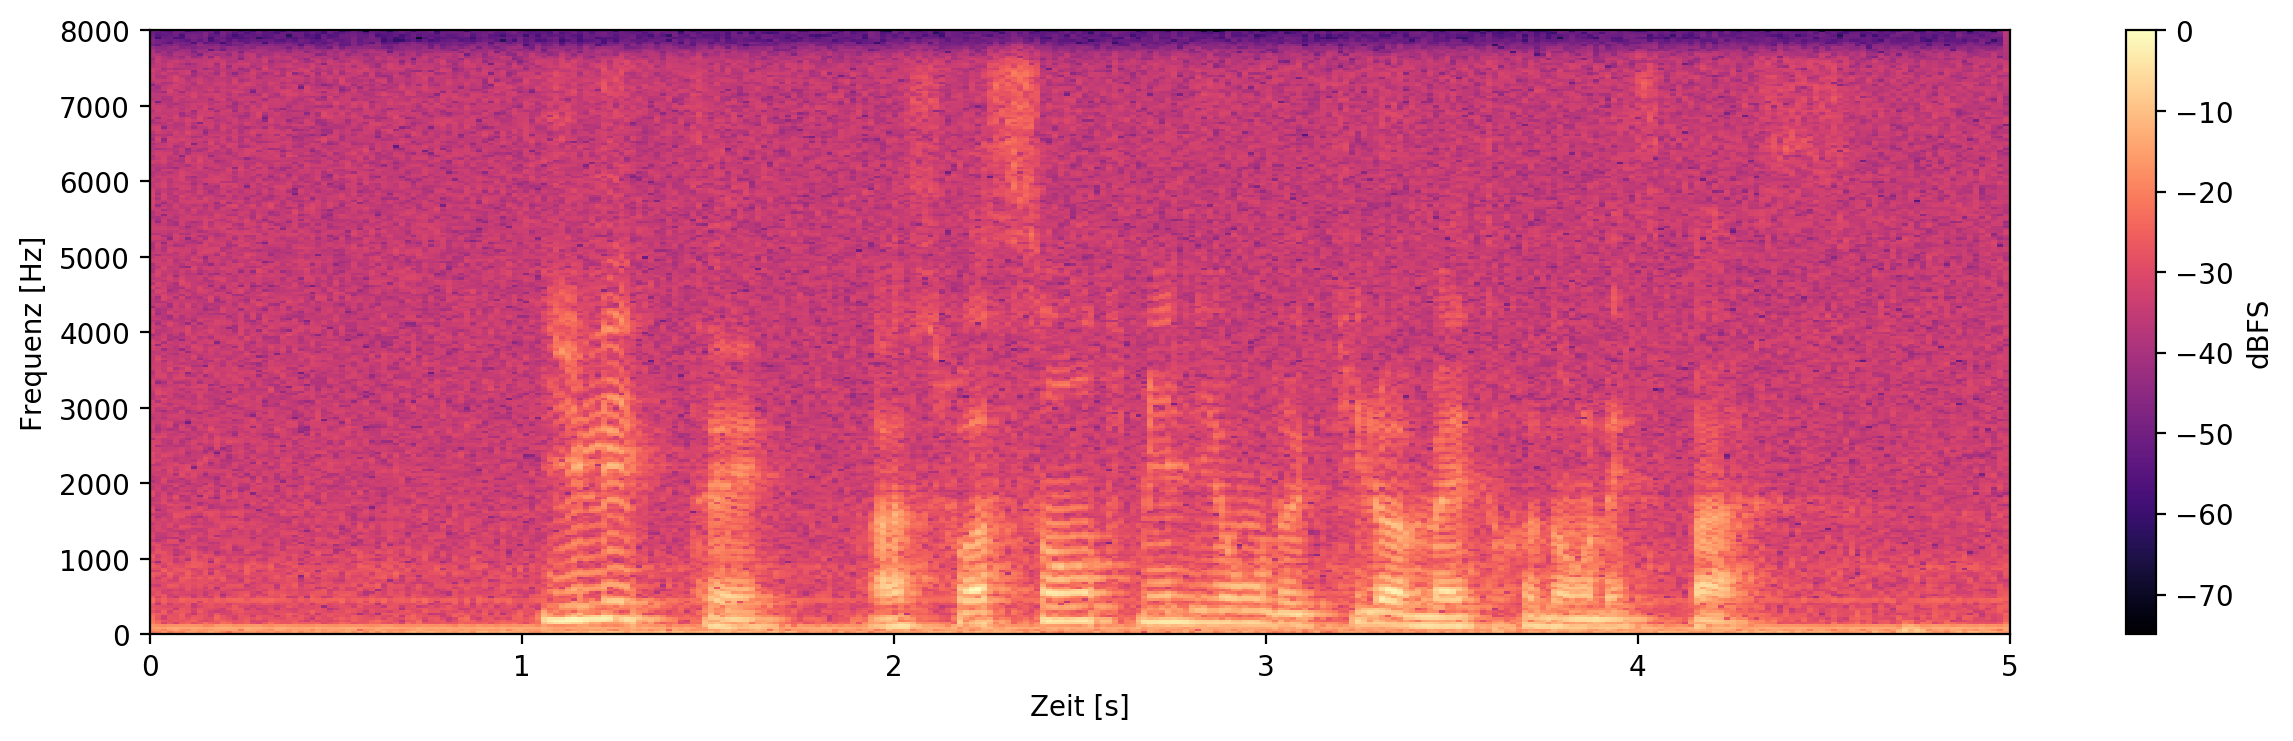
\includegraphics[width=0.8\textwidth]{assets/audio_linear.png}
		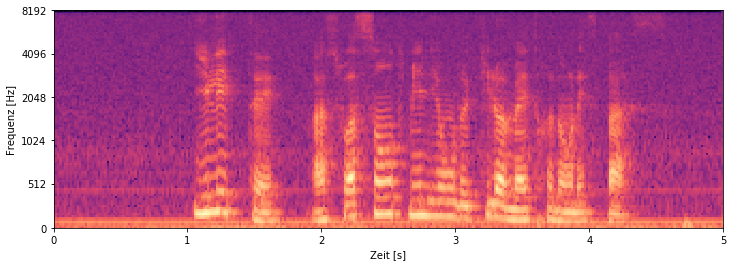
\includegraphics[width=0.8\textwidth]{assets/audio_mel.png}
	\centering
	\caption{Audio-Preprocessing: \textit{(oben)} Rohe Schallwelle, \textit{(mitte)}
		     Dezibel-Spectrogramm, 
		     \textit{(unten)} Mel Dezibel-Spectrogramm}
	\label{img:preprocessing}
\end{figure}
Spektrogramme \index{Spektrogramme}sind grafische Darstellungen eines Hörsignals nach der Anwendung der Fourrier-Transformation\parencite[]['Spectrograms']{fourrier}, ersichtlich in Abbildung \ref{img:preprocessing} \textit{(Mitte)}. Sie zeigen die Intensität der vorhandenen Frequenzen über die Zeit. Die Lautstärke der Frequenzen wird zuerst in die Logarithmische Dezibel-Skala umgerechnet. Die Einheit dBFS (\textit{Decibels relative to full scale}) gibt die Lautstärke relativ zur maximalen Lautstärke (0 dBFS) an. Es hat sich empirisch gezeigt, dass die Wahl der Dezibel-Skala einen positiven Effekt auf die Modelle hat. In der Praxis wird das Spektrogramm am Schluss noch normiert. Frequenzen über 10kHz können abgeschnitten werden, da menschliche Sprache grössten Teils darunter abläuft \parencite{tenkHz}. Im Spektrogramm lassen sich mit dem Auge Muster erkennen und unterscheiden. Daraus folgt die Idee für die Klassifizierung Bilderkennungsmethoden zu verwenden. Der visuelle Charakter der Spektrogramme erlaubt zum Beispiel das Verwenden von \textit{2D Convolutional Neural Networks}.

\subsubsection{Mel Filtering} \index{Mel Filtering}

Spektrogramme haben relativ viele Datenpunkte und sind deshalb recht aufwändig zu verarbeiten. Ein weiter \textit{preprocessing} Schritt wird deshalb oft angewendet: \textit{Mel Filtering}\parencite{mel}. Die Frequenzen werden dabei in grössere Eimer gepackt. Unter 1kHz sind die Eimer linear verteilt und darüber logarithmisch, siehe Abbildung \ref{img:preprocessing} \textit{(unten)}. Das Modell entspricht unserer Hörfähigkeit, die recht präzise unter 1kHz arbeitet, höhere Frequenzen aber schlecht unterscheiden kann \parencite{tenkHz}. 

\subsubsection{Implementation}

Die oben genannten Transformationen können vor dem Training direkt auf die Daten angewendet und abgespeichert werden. Diese Prozedur müsste aber bei jedem Experiment mit neuen Hyperparametern für das Spektrogram, wiederholt werden. Um flexibel experimentieren zu können, müssen die Daten deswegen unbedingt in ihrer rohen Form bleiben. 

Anstatt die Transformationen selber zu implementieren, wird ein Framework verwendet. In diesem Fall bietet sich an \textit{kapre}\parencite{kapre} an. Mit Kapre lassen sich während dem Training die Daten in Echtzeit verarbeiten. Das Training dauert dabei aber 20\% länger. Konkret verhält sich \textit{kapre} wie eine Schicht vor dem eigentlichen Neuronalen Netzwerk.
\begin{figure}[hbt]
	\centering
		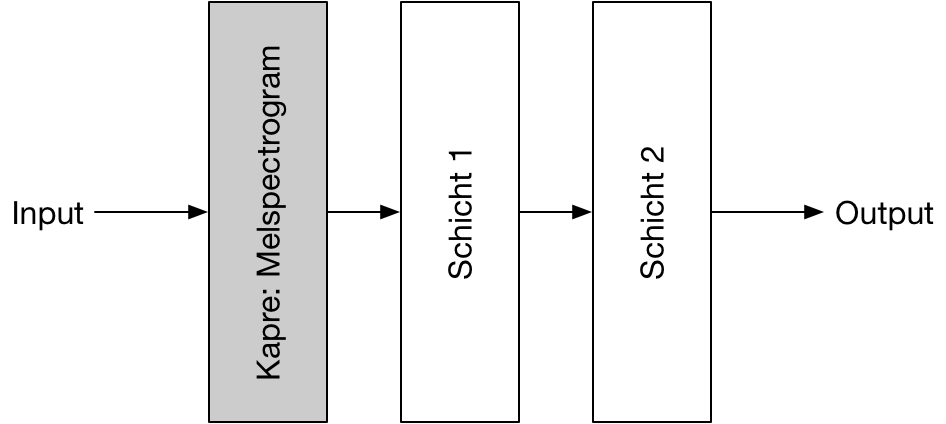
\includegraphics[width=0.6\textwidth]{assets/kapre.png}
	\centering
	\caption{\textit{Kapre}\parencite{kapre} als Schicht}
	\label{img:kapre}
\end{figure}

